\documentclass{article}

% if you need to pass options to natbib, use, e.g.:
% \PassOptionsToPackage{numbers, compress}{natbib}
% before loading nips_2017
%
% to avoid loading the natbib package, add option nonatbib:
% \usepackage[nonatbib]{nips_2017}

\PassOptionsToPackage{numbers, compress}{natbib}
\usepackage{nips_2017}

% to compile a camera-ready version, add the [final] option, e.g.:
% \usepackage[final]{nips_2017}

\usepackage[utf8]{inputenc} % allow utf-8 input
\usepackage[T1]{fontenc}    % use 8-bit T1 fonts
\usepackage{hyperref}       % hyperlinks
\usepackage{url}            % simple URL typesetting
\usepackage{booktabs}       % professional-quality tables
\usepackage{amsfonts}       % blackboard math symbols
\usepackage{nicefrac}       % compact symbols for 1/2, etc.
\usepackage{microtype}      % microtypography

%for matrices
\usepackage{blkarray}
\usepackage{amsmath}

\usepackage{graphicx}
\usepackage{caption}
\usepackage{subcaption}

\usepackage[svgnames, table]{xcolor} % Enabling colors by their 'svgnames'

% define custom commands
\definecolor{commentPJA_color}{rgb}{1.0,0.0,0.8}
\newcommand{\commentPJA}[1]{{\textcolor{commentPJA_color}{PJA: #1}}}


% define custom commands
\definecolor{commentLP_color}{rgb}{1.0,0.0,0.8}
\newcommand{\commentLP}[1]{{\textcolor{commentLP_color}{LP: #1}}}


% define custom commands
\definecolor{commentAP_color}{rgb}{1.0,0.0,0.8}
\newcommand{\commentAP}[1]{{\textcolor{commentAP_color}{AP: #1}}}

% define custom commands
\definecolor{commentRJ_color}{rgb}{1.0,0.0,0.8}
\newcommand{\commentRJ}[1]{{\textcolor{commentRJ_color}{RJ: #1}}}


\newcommand{\mb}[1]{\mathbf{#1}}
\newcommand{\bs}[1]{\boldsymbol{#1}}
\newcommand{\mvec}[1]{\mathbf{#1}}

\title{Givens Transform Approach for Efficient Probabilistic Principle Component Analysis for Bayesian Dimensionality Reduction (GT-PPCA)}

% The \author macro works with any number of authors. There are two
% commands used to separate the names and addresses of multiple
% authors: \And and \AND.
%
% Using \And between authors leaves it to LaTeX to determine where to
% break the lines. Using \AND forces a line break at that point. So,
% if LaTeX puts 3 of 4 authors names on the first line, and the last
% on the second line, try using \AND instead of \And before the third
% author name.

\author{
  David S.~Hippocampus\thanks{Use footnote for providing further
    information about author (webpage, alternative
    address)---\emph{not} for acknowledging funding agencies.} \\
  Department of Computer Science\\
  Cranberry-Lemon University\\
  Pittsburgh, PA 15213 \\
  \texttt{hippo@cs.cranberry-lemon.edu} \\
  %% examples of more authors
  %% \And
  %% Coauthor \\
  %% Affiliation \\
  %% Address \\
  %% \texttt{email} \\
  %% \AND
  %% Coauthor \\
  %% Affiliation \\
  %% Address \\
  %% \texttt{email} \\
  %% \And
  %% Coauthor \\
  %% Affiliation \\
  %% Address \\
  %% \texttt{email} \\
  %% \And
  %% Coauthor \\
  %% Affiliation \\
  %% Address \\
  %% \texttt{email} \\
}

\begin{document}
% \nipsfinalcopy is no longer used

\maketitle

\begin{abstract}
We develop scalable and flexible Probabilistic Principal Component Analysis (PPCA) methods for determining posterior distributions of spanning frames based on a Givens Representation of the PCA which we term (GT-PPCA).  This addresses significant challenges that arise with latent variable in a traditional formulation of PPCA.  For sampling posterior distributions we develop Hamiltonian Monte-Carlo Methods (HMC) for sampling on the Stiefel Manifold the PCA orthogonal frame sets.  We demonstrate our approach on several challenging example problems including tests problems XYZ and problems arising in  our recent work on understanding medical patient data associated with coagulopathy (factors influencing blood clotting).  We show our methods provides ways to identify when data sets contain a mixture of low dimensional structures that would not be resolved with traditional PCA approaches.  We further show how our approach can be used to develop heirarchical models in terms of low dimensional structures learned from the data sets or to develop prior distributions useful in generalizing low dimensional structures to new settings.  To facilitate use of our GT-PPCA method we provide a package with the widely-used Stan statistics package.  
\end{abstract}

%%%%%%%%%%%%%%%%%%%%%%%%%
\section{Introduction}
%%%%%%%%%%%%%%%%%%%%%%%%%

%\commentPJA{For later, Try to bring forth the novelty of our methods earlier in introduction while explaining the traditional PCA.  Best to have first draft and then streamline at the end after all materials together.}

Principal Component Analysis (PCA) is a widely used dimensionality-reduction tool for exploratory analysis and modeling in both the natural and social sciences. By factorizing an empirical covariance matrix into a product of low rank matrices, PCA effectively finds a low dimensional subspace that describes the dataset in terms of the latent factors.  These latent factors are given by the columns of the low rank factorization.  Geometrically, traditional PCA can be interpreted as providing a point estimate of a low dimensional hyper-plane that is closest to a cloud of data points. PCA  and other variants are also routinely applied to binary or integer valued matrices, such as item response tables in recommendation systems or graph adjacency matrices arising in network science \citep{lee2001algorithms, collins2001generalization}.

Probabilistic PCA (PPCA) \citep{tipping1999probabilistic} posits a probabilistic generative model that is equivalent to PCA in the limit of decreasing noise \citep[chapt.~12.2]{murphy2012machine}. This probabilistic approach is attractive because it enables a straightforward methodology, via Bayesian inference, to quantify the uncertainty in our estimates (to prevent overfitting) and conduct hypothesis testing. For example, given high dimensional medical data for patients with two different type of injuries, it would be desirable to find posterior distributions of low-dimensional subspaces that describe the data, then find the probability given the data that these subspaces are different for the two groups of patients. While uncertainty quantification of the latent factors in PPCA has been explored in the literature \citep{hoff2009simulation,brubaker2012family, byrne2013geodesic}, there are currently no out-of-the-box solutions available to researchers. 

In addition to enabling uncertainty quantification and hypothesis testing, probabilistic models are amenable to expansion and can serve as modules within larger probabilistic graphical models. This is important in real-world settings where we seek to utilize any known prior information in our inference or when true generative models do not necessarily follow the simple generative process set forth by PPCA. If we believe our latent factors to be sparse, we can add Laplace or Cauchy priors to our PPCA model yielding a probabilistic sparse PCA\citep{zou2006sparse}. Following the medical example, we may believe subspaces for different groups of patients come from some common prior distribution of subspaces, in which case we can build a hierarchical model to do transfer learning. Similarly, we can expand the PPCA graphical model to conduct non-linear dimensionality reduction via Mixtures of Factor Analyzers \citep{ghahramani1996algorithm}. To handle binary or discrete data we can expand PPCA using a link function as in Bayesian Exponential Family PCA (BXPCA) \citep{mohamed2009bayesian}.

While expanded PPCA models have shown promise on a variety of problems, they have not been fully explored because their implementation remains elusive, and most inference schemes such as Expectation Maximization (EM) only provide point estimates. The availability of PPCA in a simple framework for building probabilistic graphical models like Stan \citep{carpenter2016stan} would allow rapid building and prototyping of such models in a fully Bayesian way that provides uncertainty around any point estimates.

\paragraph{Bayesian inference of orthonormal matrices} Many of the difficulties in conducting full Bayesian inference on PPCA and related models stem from having to infer one or more unknown orthonormal matrix parameters.  This is difficult because orthonormal matrices form a rather particular subset (or submanifold) of all possible realizable matrices, analogous to three-dimensional unit vectors lying on the sphere (a submanifold of $\mathbb{R}^3$). This yields a probability distribution on a sub-manifold within the full space of matrices that has a non-trivial geometry.  More specifically, the prior and posterior distributions of an orthonormal matrix $W$ must have support over the set of $n \times p$ orthonormal matrices.  This is known as the Stiefel manifold and denoted $V_{n,p}$ \citep{muirhead2009aspects}.

When first considering this problem, it may seem that this geometry may rule out a straightforward use of two of the most prominent techniques for posterior inference posterior inference, Markov Chain Monte Carlo (MCMC) and Variational Inference (VI).  Intuitively, for MCMC, we have no way of guaranteeing that a chain over $W$ will explore only valid regions of parameter space that satisfy the orthonormality constraints. Similarly for Variational Inference, positing a common variational posterior distribution such as a Gaussian over the elements of $W$ is sure to lead to posteriors that assign mass to invalid regions of parameter space.

\paragraph{Transformed random variables} Posterior distributions for constrained parameters in probabilistic graphical models are routinely inferred by transforming such parameters to an unconstrained space and seeking posterior distributions over the transformed parameter~\citep{carpenter2016stan, kucukelbir2014fully}. This requires a smooth one-to-one transformation $f: \mathrm{supp}(z_\mathrm{constr}) \to \mathbb{R}^D$, where $\mathrm{supp}(z_\mathrm{constr})$ is the support of the constrained random variable $z_\mathrm{constr}$. To our knowledge, no such transformation has been proposed to map orthonormal matrices to a comparable unconstrained space.

In this paper we draw on techniques from Differential Geometry and Numerical Analysis to introduce a novel and geometrically elegant way to represent orthonormal matrices.  In our approach we express orthonormal matrices in terms of a sequence of fundamental rotations through given angles. This gives insight into the geometry of the Stiefel manifold, and results in a transform we call the Givens Transform, that maps orthonormal matrices to an unconstrained space. We apply the Givens Transform to inference of PPCA-based models, and collectively refer to this as GT-PPCA.

\paragraph{GT-PPCA} GT-PPCA is straightforward to implement in stand-alone inference schemes, but is particularly useful in the context of probabilistic programming framework like Stan \citep{carpenter2016stan}, where we can use it for uncertainty quantification and hypothesis testing of PPCA models, as well as extending PPCA to more complex probabilistic graphical models, two previously intractable tasks. We provide Stan code for our example models allowing for use and expansion by researchers and scientists out-of-the-box. We demonstrate how inference of these models in Stan yields good empirical performance on large probabilistic graphical models that were previously intractable to implement especially if fully-Bayesian posterior analysis is desired. Specifically we present a hierarchical subspace model for grouped, multi-view medical data and a PPCA Hidden Markov Model (HMM) for disease-network data.

In addition to opening the door for straightforward implementation of large PPCA models, GT-PPCA yields insight in to novel and useful ways to work with and interpret our models.  For instance, the elegant geometric representation lets us see how by limiting the range of the parameters in GT-PPCA, we can naturally avoid issues of unidentifiability and multi-modal posteriors that arise in other methods.  GT-PPCA also allows us new and creative ways to generate and use prior distributions on orthonormal matrices.  In the setting of using the matrix directly this task has previously been rather complicated and rather intractable for even small problem sizes.  This is linked to the difficulty of evaluating densities of orthonormal matrix distributions in other representations.  As we shall discuss in more detail, our GT representation provides a rather natural way to specify prior distributions comparable to the Matrix Langevin prior \citep{muirhead2009aspects}.

\paragraph{Related work} While previous authors have developed methods for posterior sampling of distributions orthonormal matrices, these methods can at times suffer from numerical issues, they are difficult to implement on large probabilistic graphical models, and they can not be used in any general inference scheme such as VI or Maximum A-Posteriori (MAP) estimation like GT-PPCA can. \citet{brubaker2012family} and 
\citet{byrne2013geodesic} used separate approaches to modify the Leap-Frog integrator typically used in Hamiltonian Monte Carlo (HMC), so that Hamiltonian exploration, and thus MCMC samples of posteriors, satisfied any necessary constraints at all times. Specifically,~\citet{brubaker2012family} uses the SHAKE integrator \citep{leimkuhler2004simulating} to simulate Hamiltonian dynamics and generate proposals. The integrator works by repeatedly taking a step forward that may be off the manifold using ordinary leap frog, then projecting back down to the nearest point on the manifold. This projection is done via Newton iterations, which may converge to the wrong local minimum in practice or perhaps not converge at all, possibly jeopardizing the ergodicity of a Markov Chain, and the integrity of samples~\citep{betancourt2017divergences}. \citet{byrne2013geodesic}~took a different approach, exploiting the fact that closed form solutions are known for the geodesic equations over the Stiefel manifold in the embedded coordinates, $W$. While this method is completely explicit, requiring no Newton iterations, in practice we found that for larger step sizes, the integrator steps off the Stiefel manifold, due to the numerical imprecision of the matrix exponential function. Because these methods use modified integrators for constrained parameters, in practice they require keeping track of the support of each variable and which type of integrator to use on each variable. This adds an extra layer of implementation complexity, especially for large complex probabilistic graphical models, that makes it difficult to implement these methods within a probabilistic programming language such as Stan. This precludes the rapid prototyping and building of models as well as the flexibility to use different inference schemes that Stan provides. Lastly, we remark that for inference on orthonormal matrices, these methods can lead to multi-modal posteriors, that can be avoided in a straight-forward way using the Givens transform.

\paragraph{Paper outline} We give a brief overview of probabilistic dimensionality reduction in Section~\ref{Probabilistic dimensionality reduction}. We discuss the geometry of the Stiefel Manifold in Section~\ref{geometry}, before finally introducing the Givens Transform (GT) in Section~\ref{Givens}. Finally, we present various empirical studies where we used GT-PPCA in Stan for practical uncertainty quantification and hypothesis testing, as well as for building complex probabilistic graphical models.

%%%%%%%%%%%%%%%%%%%%%%%%%

%%%%%%%%%%%%%%%%%%%%%%%%%
%%%%%%%%%%%%%%%%%%%%%%%%%
%%%%%%%%%%%%%%%%%%%%%%%%%
\section{Probabilistic Principle Component Analysis (PPCA)} \label{Probabilistic dimensionality reduction}
%%%%%%%%%%%%%%%%%%%%%%%%%
%%%%%%%%%%%%%%%%%%%%%%%%%
%%%%%%%%%%%%%%%%%%%%%%%%%

In probabilistic principle component analysis (PPCA) one starts by considering a collection of data points in a typically high-dimensional vector space and seeks to find a posterior distribution over a reduced representations of the data in the form of a lower dimensional subspace.  The central postulate is that for a data vector $\mathbf{x} \in \mathbb{R}^n$ there exists an unknown low-dimensional latent representation $\mathbf{z} \in \mathbb{R}^p$ where $p < n$, (ideally with $p \ll n$).  The two representations are related to each other by a single unknown linear transformation $\mathbf{x} \rightarrow \mathbf{z}$.  Mathematically, we consider a finite collection of sampled data vectors $\mathbf{x}_i \in \mathbb{R}^n$, $i = 1, \cdots, N$ and try to estimate this subspace.  Formally, PPCA consists of the following generative process

\begin{eqnarray}
\label{eq:PpcaGenerativeProcess}
p(\mb{z}_i) &\sim& \mathcal{N}_p(0, I) \nonumber\\
p(\mb{x}_i | \mb{z}_i, W, \Lambda, \sigma^2) &\sim& \mathcal{N}_n(W \Lambda \mb{z}_i, \sigma^2 I).
\end{eqnarray}
The $W$ is an $n \times p$ orthonormal matrix and $\Lambda$ is a $p \times p$ diagonal matrix with positive elements.  For simplicity in our presentation of PPCA, we have assumed here that the data has only zero mean but the more general case can also readily be considered \citep[chapt.~12.1]{murphy2012machine}. 

\paragraph{Quantifying uncertainty}
Inference for PPCA is typically conducted by obtaining a point estimate for $W$ via a closed-form estimator, or for expanded PPCA models via (EM) \citep[chapt.~12.2]{murphy2012machine}, neither of which provide a notion of uncertainty for our point estimates. Without information regarding the uncertainty of our estimates these point estimates could be far from the true value of $W$ and thus mislead our conclusions, especially for larger models and/or when there is relatively little data available. Furthermore, point estimates do now allow for hypothesis testing e.g. statistically testing whether two different groups of observations lie in the same subspace. We show with examples how GT-PPCA in Stan makes it easy achieve these tasks as we show in section \ref{examples}.

\paragraph{Expanding models}
As alluded to previously, PPCA generative model can be flexibly expanded in several ways as modelers see fit. To build a probabilistic sparse PCA, one can place a Laplace or Cauchy prior over the elements of $W$. If we have meaningfully grouped data, such as data from hospital patients with different types of injury, it might be desirable to designate a separate $W$ parameter (subspace) for each group, then place prior over these subspaces to garner the benefits of hierarchical modeling \citep[chapt.~5]{gelman2014bayesian}. \citet{mohamed2009bayesian} showed that we can model non-Gaussian data, $\mb{x}_i$, by replacing equation \ref{eq:PpcaGenerativeProcess} with an exponential family member whose natural parameters are given by $\mathrm{Expon}(W\Lambda \mb{z}_i)$ where $\mathrm{Expon}(\cdot)$ is an appropriate link function.  Again, in the context of a probabilistic programming language such as Stan, these extensions to the base PPCA model become trivial to implement as we illustrate with examples in section \ref{examples}.

\paragraph{Importance of the Orthonormality Condition}
The orthonormal constraint on the matrix $W$ plays an important role in obtaining robust methods for making inferences in probabilistic PCA because it alleviates identifiability and numerical issues.  If one were to relax the orthonormality constraint the likelihood function would assign identical probability to a whole equivalence class of matrices $W \sim V$ where the span is the same linear subspace $\mbox{span}\{W\} = \mbox{span}\{V\}$ \citet[chapt.~12.1.3]{murphy2012machine}.  Besides resulting in an unidentifiable model, in practice this presents a number of major challenges.  This first is that the matrices in a given equivalence class are not all equally well-conditioned numerically and round-off errors and truncation errors become problematic in practical calculations.  Secondly, these issues with the representation further manifest in the log-likelihood objective function where regions arise of particularly large curvature as pointed out by \citep{holbrook2016bayesian}.  This causes significant numerical issues for variational inference (VI) in nonlinear optimization methods and in Monte-Carlo (MC) approaches with samplers having slow mixing times \citep{holbrook2016bayesian}. We note that, while most identifiability issues and numerical issues are alleviated by constraining inference to orthonormal matrices, the PPCA likelihood is equivalent for an orthonormal matrix $W$ and any permutation of the columns of $W$ being negative as pointed out by both \citet[chapt.~12.1.3]{murphy2012machine} and  \citet{holbrook2016bayesian}. As such, even the methods of \citet{brubaker2012family} and \citet{byrne2013geodesic} will lead to multi-modal posteriors, that can be avoided in a straight-forward way by appealing to insights revealed by the Givens Transform, as we explain in Section~\ref{Givens}.


%%%%%%%%%%%%%%%%%%%%%%%%%
%%%%%%%%%%%%%%%%%%%%%%%%%
%%%%%%%%%%%%%%%%%%%%%%%%%
\section{Geometry of the Stiefel Manifold} \label{geometry}
%%%%%%%%%%%%%%%%%%%%%%%%%
%%%%%%%%%%%%%%%%%%%%%%%%%
%%%%%%%%%%%%%%%%%%%%%%%%%

The set of $n\times p$ orthonormal matrices $V_{n,p}$, form a sub-manifold in the space of general $n \times p$ matrices known as the Stiefel Manifold \citep{muirhead2009aspects} and formally defined as

\begin{equation}
V_{n,p} := \{Y \in \mathbb{R}^{n \times p}: YY^T = I \}.
\end{equation}

Intuitively, the elements of $V_{n,p}$ can be thought of not as orthonormal matrices, but as $p$-frames which are comprised of $p$ orthonormal vectors that lie in $n$-dimensional space. To move about the Stiefel manfiold, one can rigidly rotate the vectors in the $p$-frame about any combination of axes an arbitrary number of times. In the case where $n = 3$ and $p = 2$, this is almost identical to sphere (Figure \ref{fig:StiefelGeom}), but with an extra angle, $\theta_{23}$ that controls how much the second basis vector is rotated about the first. For a three-dimensional set of points forming a flat, pancake-like cloud, PPCA can be thought of as finding the best $2$-frame that aligns with this cloud.

\begin{figure}
    \centering
    \begin{subfigure}[b]{0.3\textwidth}
        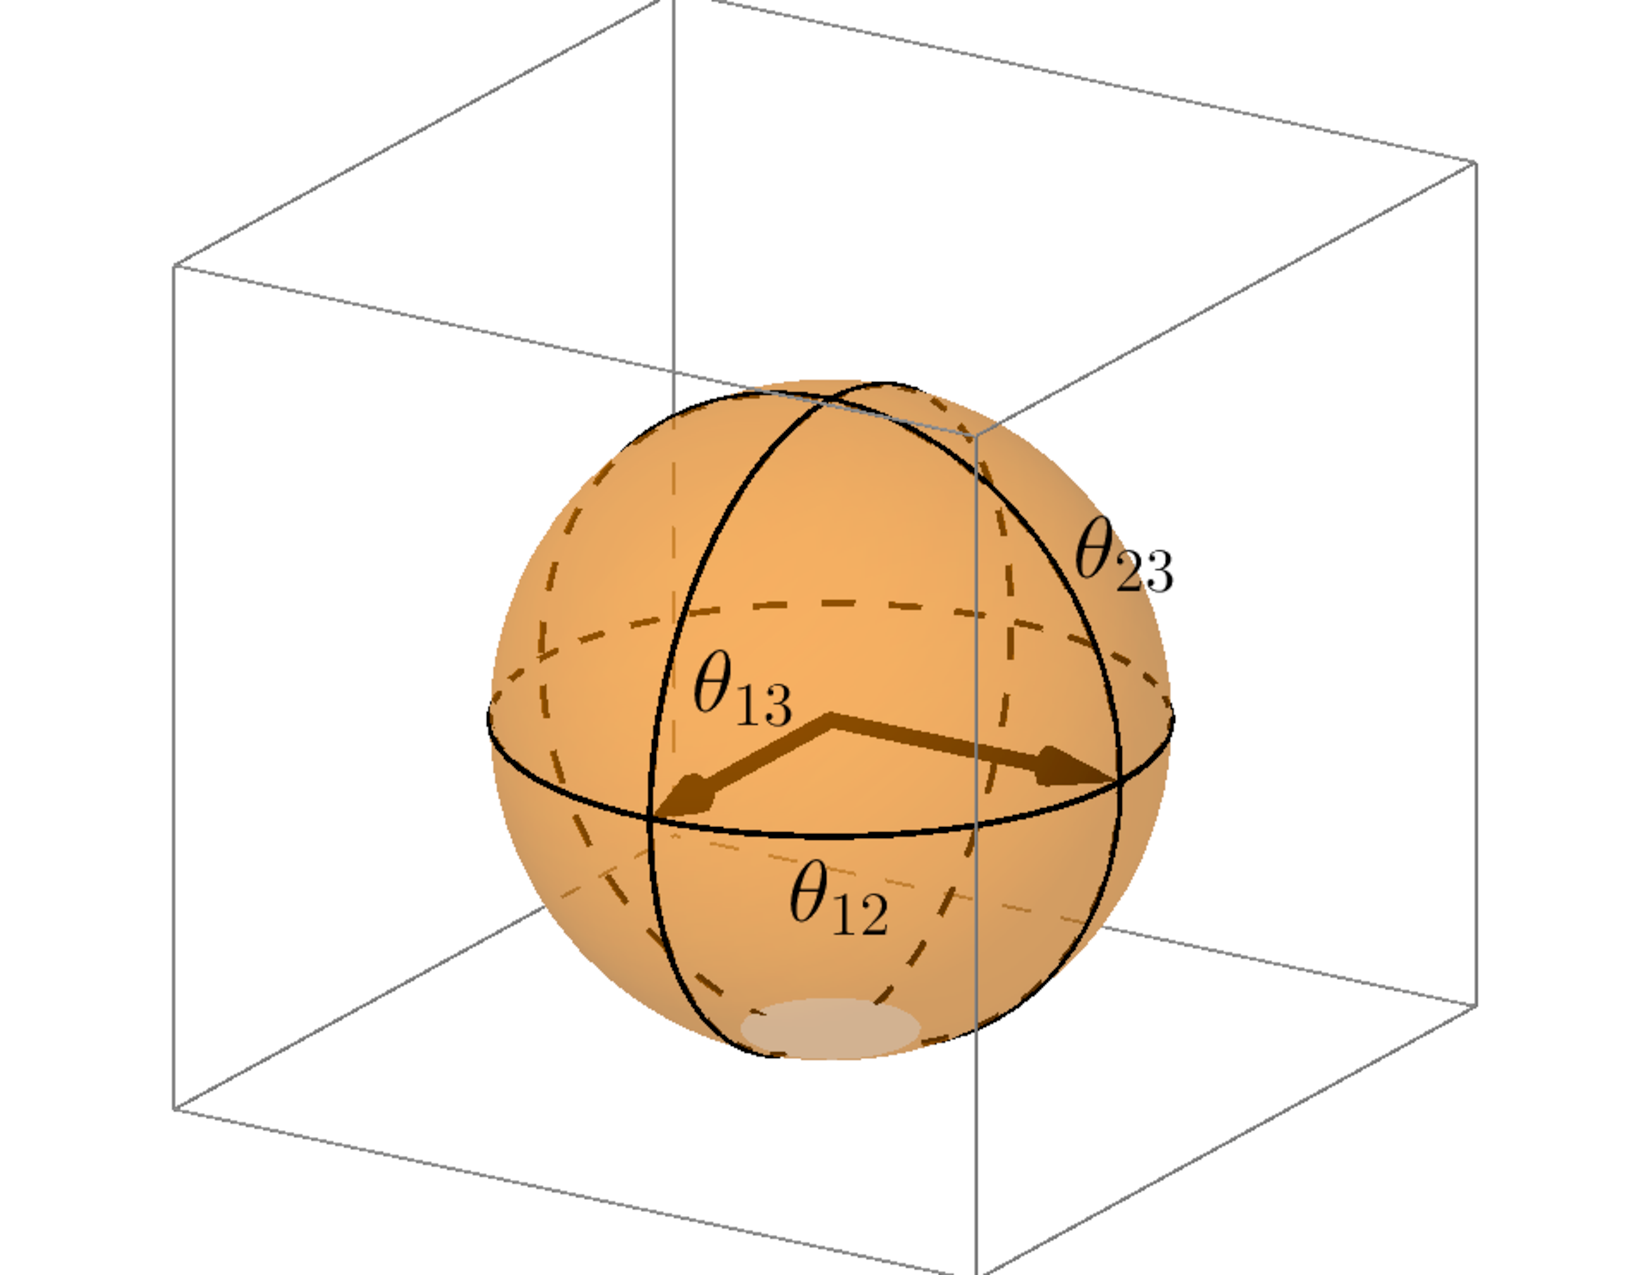
\includegraphics[width=\textwidth]{StiefelGeom.pdf}
        \caption{}
        \label{fig:StiefelGeom}
    \end{subfigure}
    ~ %add desired spacing between images, e. g. ~, \quad, \qquad, \hfill etc. 
      %(or a blank line to force the subfigure onto a new line)
    \begin{subfigure}[b]{0.3\textwidth}
        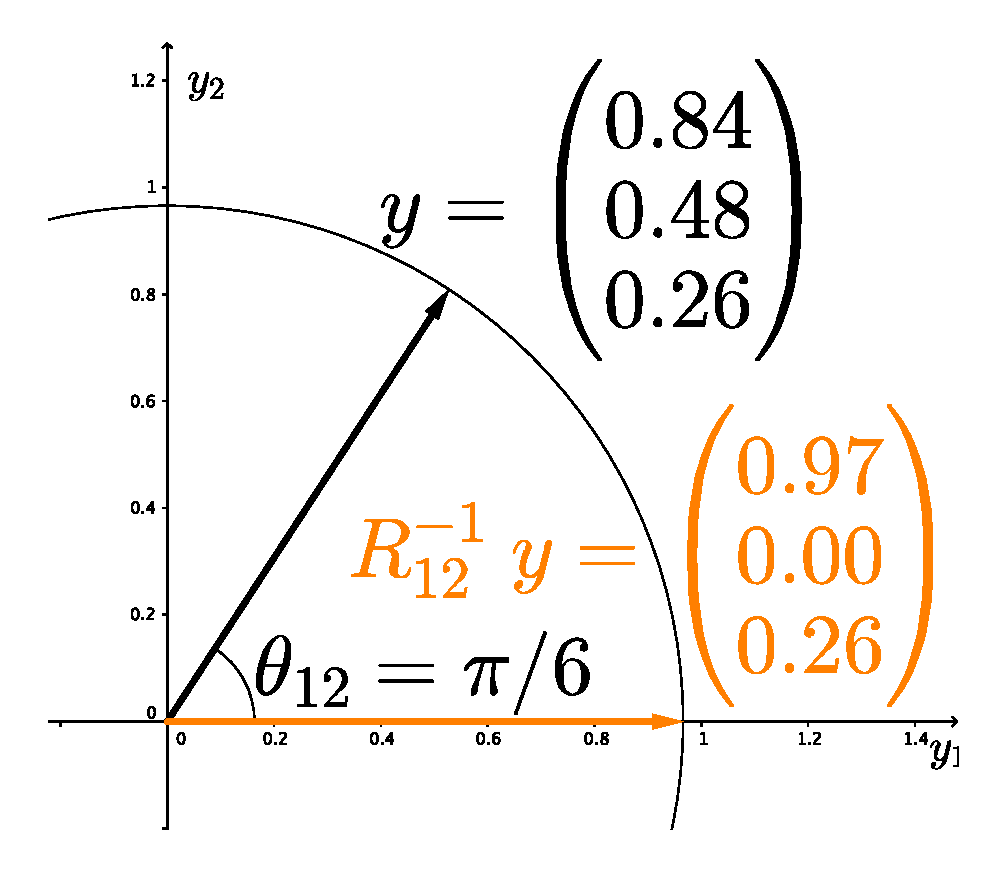
\includegraphics[width=\textwidth]{GivensReduction.pdf}
        \caption{}
        \label{fig:GivensReductionm}
    \end{subfigure}
    ~ %add desired spacing between images, e. g. ~, \quad, \qquad, \hfill etc. 
    %(or a blank line to force the subfigure onto a new line)
    \begin{subfigure}[b]{0.3\textwidth}
        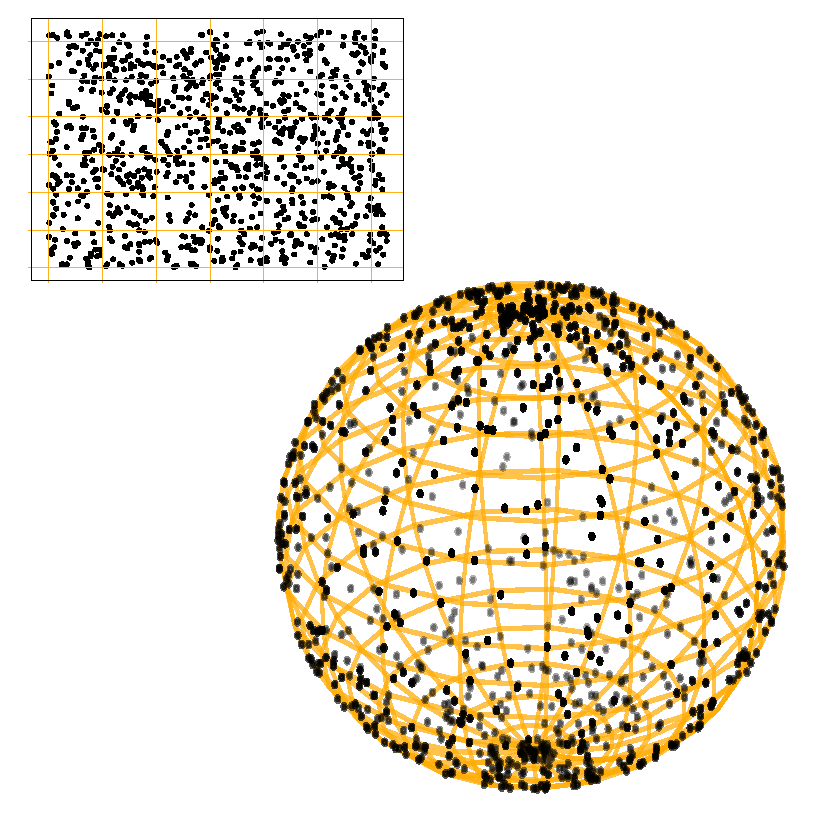
\includegraphics[width=\textwidth]{AreaForm.pdf}
        \caption{}
        \label{fig:AreaForm}
    \end{subfigure}
    \caption{Visualizing the Givens Transform. (a) How the Givens Reduction ``zeros out'' a column vector. (b) A geometric view of the Stiefel manifold, two-frame in three dimensions. (c) Sampling without a proper measure adjustment.}\label{fig:Givens}
\end{figure}
 
While $n \times p$ orthonormal matrices are represented by $np$ elements, the Stiefel Manifold $V_{n,p}$, has an intrinsic dimension of $np-p(p+1)/2$. This arises from the constraints on the columns of the matrix that impose orthonormality.  This dimensionality can be seen by observing, that the first column of $Y \in V_{n,p}$ must have norm one and hence has one constraint placed on it. The second column must also have norm one and also must be orthogonal to the first column hence with two constraints placed on it.  Continuing to the third column through the $n^{th}$ one arrives at the conclusion that each point of the Stiefel Manifold has only $np - (1+2+\cdots+p) =np-p(p+1)/2$ degrees of freedom.  The Givens transform can be thought of as an $np-p(p+1)/2$-dimensional set of coordinates $\Theta$, that represent elements of the Stiefel manifold.

%%%%%%%%%%%%%%%%%%%%%%%%%
%%%%%%%%%%%%%%%%%%%%%%%%%
%%%%%%%%%%%%%%%%%%%%%%%%%
\section{Givens Transform (GT) approach to PPCA (GT-PPCA)} \label{Givens}
%%%%%%%%%%%%%%%%%%%%%%%%%
%%%%%%%%%%%%%%%%%%%%%%%%%
%%%%%%%%%%%%%%%%%%%%%%%%%

For several types of constrained parameters, posterior distributions are in practice rather routinely inferred using both MCMC and VI by transforming the constrained variables to an unconstrained space using a one-to-one mapping $T: \mathrm{supp}(z_\mathrm{constr}) \to \mathbb{R}^D$, where $\mathrm{supp}(z_\mathrm{constr})$ is the support of the constrained random variable $z_\mathrm{constr}$. One can obtain a posterior over the unconstrained parameter that corresponds to the original constrained parameter of interest, then map inferences back to the original constrained space. This procedure requires computing the Jacobian, $J_{T^{-1}}$ of the transformation, to obtain $f_{Y}(y) = f_{z_\mathrm{constr}}(T^{-1}(y)) J_{T^{-1}}(y)$ where $Y$ is an unconstrained random variable with probability density function (PDF) $f_Y$ and $f_{z_\mathrm{constr}}$ is the probability density of $z_\mathrm{constr}$, which for PPCA comes from equation \ref{eq:PpcaGenerativeProcess}. The extra Jacobian term accounts for how the a unit volume under the transformation changes \citep{kucukelbir2014fully}. Without this extra Jacobian factor, inference between the two spaces is incomparable. For example, uniformly sampling in spherical coordinates (unconstrained space) does not correspond to uniformly sampling on the sphere (constrained space), unless we include an appropriate term accounting for how volumes are warped under the transformation (see Figure \ref{fig:AreaForm}).  Conducting inference in a transformed space is most notably used in ADVI and Stan's HMC routines \citep{carpenter2016stan, kucukelbir2014fully}. In sub-section \ref{GivensSub} we briefly discuss Givens Reductions, motivating the Givens Transform. In sub-section \ref{geomGivens} we discuss geometric aspects of the Givens transform such as avoiding multi-modality and including a term that measures how volume is changed under the transform that is analogous to the Jacobian described above.

%%%%%%%%%%%%%%%%%%%%%%%%%
\subsection{Givens Reductions and the Givens Transform}\label{GivensSub}
%%%%%%%%%%%%%%%%%%%%%%%%%

\commentPJA{Give a basic description of the background on Givens reductions of a matrix that we can refer to with additional details than we need in the main text.}

%%%%%%%%%%%%%%%%%%%%%%%%%
\subsection{Geometry of the Givens Transform}\label{geomGivens}
%%%%%%%%%%%%%%%%%%%%%%%%%

limiting angles and area form.

\commentPJA{Discuss the basic differential geometry of the Steifel Manifold and how we handle these various issues.  Degenerate regions and metric factors (Jacobians).  Discuss how we use "multi-coordinate charts" when necessary to avoid being close to regions with bad metric factors and degeneracy, etc...}



%%%%%%%%%%%%%%%%%%%%%%%%%
%%%%%%%%%%%%%%%%%%%%%%%%%
%%%%%%%%%%%%%%%%%%%%%%%%%
\section{Empirical Studies} \label{examples}
%%%%%%%%%%%%%%%%%%%%%%%%%
%%%%%%%%%%%%%%%%%%%%%%%%%
%%%%%%%%%%%%%%%%%%%%%%%%%

%%%%%%%%%%%%%%%%%%%%%%%%%
\subsection{Synthetic Data}
We generated a synthetic, three-dimensional dataset that lies on a two-dimensional plane with $N =15$ observations according the generative process of PPCA \ref{eq:PpcaGenerativeProcess}. We chose $\mathrm{diag}(\Lambda) =\mathrm{diag}(1, 1)$, $\sigma^2 = 1$, and $W$ to be $I_{3,2}$ which in the Givens representation corresponds to $\theta_{12} = \theta_{13} = \theta_{23} = 0$. This example illustrates how simply running GT-PPCA in Stan can alleviate overfitting issues in the common use-case where one seeks to carry out dimensionality reduction in a low-observation regime. A standard classical PCA analysis yields the singular values $\mathrm{diag}(\hat{\Lambda}) = (1.52,\, 1.27,\, 0.77)$,  possibly suggesting that our data lie close to some two-dimensional plane, since the third singular value has a larger drop off from the first two than the second has from the first. Figure \ref{fig:MleSubspaceEstimate} illustrates geometrically a point estimate of the subspace found by PCA. This corresponds to the subspace spanned by the PCA point estimates of the latent factor loadings. Because of relatively low signal to noise ratio and modest sample size, the point estimate is drastically affected by only a few observations and is characteristically different from the flat plane, which we know to be the truth in this case. The PCA point estimate $\theta_{13}$, which if we recall from Figure \ref{fig:StiefelGeom} is the Givens Transform angle that controls the upwards tilt of the plane, is $\hat{\theta}_{13} = -0.15$. Meanwhile, posterior HMC samples from GT-PPCA in Stan yields a median value of -0.24 and a 95\% posterior interval of $(-1, 0.78)$. This lets us know that there is high uncertainty around our point estimate given the data, and suggests that any conclusions drawn from point estimates may be overfit to the data, thus protecting us from concluding false-positive results and suggesting to the experimenter that more data is needed to make a conclusive statement. Alternatively, we can incorporate any prior knowledge we have about the problem, such as knowledge about the structure of $W$ or knowledge about the $W$ of a closely related group of samples, in the form of a prior distribution of our angles in our Stan model as we do in the following subsections.

\begin{figure}
    \centering
    \begin{subfigure}[b]{0.3\textwidth}
        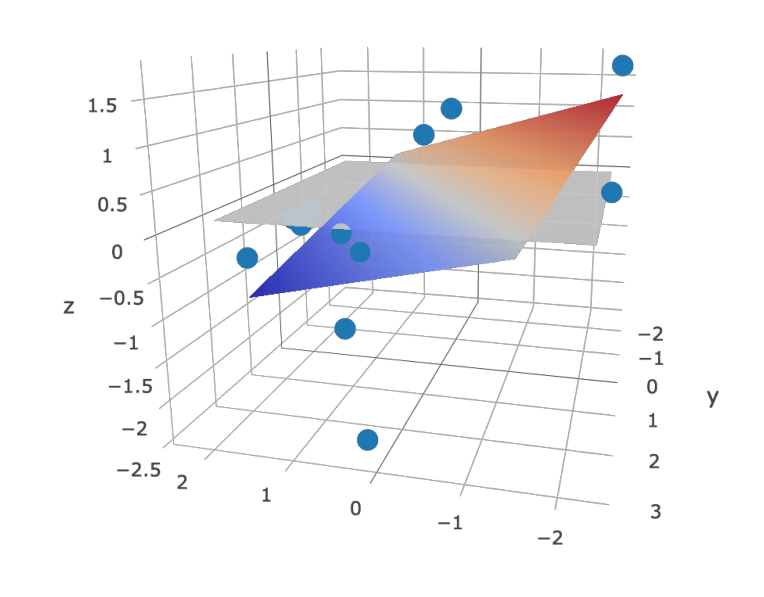
\includegraphics[width=\textwidth]{uncertainty.pdf}
        \caption{}
        \label{fig:MleSubspaceEstimate}
    \end{subfigure}
    ~ %add desired spacing between images, e. g. ~, \quad, \qquad, \hfill etc. 
      %(or a blank line to force the subfigure onto a new line)
    \begin{subfigure}[b]{0.3\textwidth}
        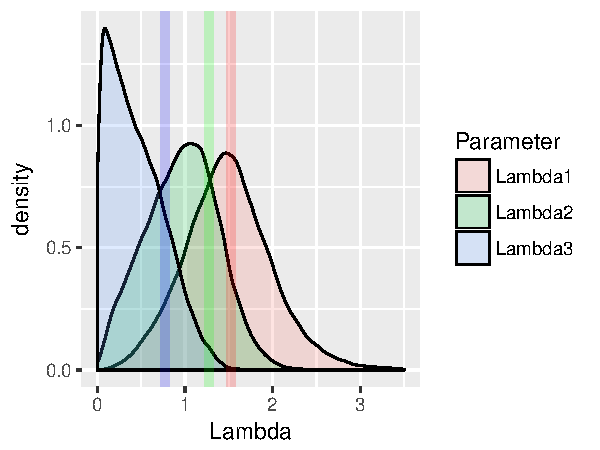
\includegraphics[width=\textwidth]{syntheticLambdaPosterior.pdf}
        \caption{}
        \label{fig:SyntheticPosteriorEstimates}
    \end{subfigure}
    ~ %add desired spacing between images, e. g. ~, \quad, \qquad, \hfill etc. 
    %(or a blank line to force the subfigure onto a new line)
    \begin{subfigure}[b]{0.3\textwidth}
        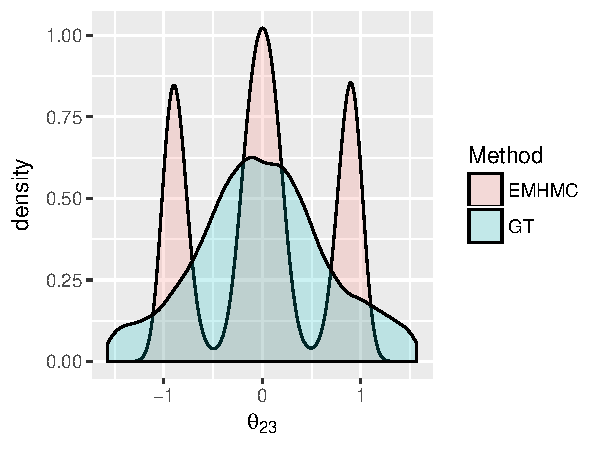
\includegraphics[width=\textwidth]{multiModal.pdf}
        \caption{}
        \label{fig:multiModal}
    \end{subfigure}
    \caption{Inferences for three-dimensional synthetic data. (a) Three-dimensional points, true subspace (grey), and classical PCA point estimate of subspace (colored). (b) Estimated densities from posterior draws of $\Lambda$ parameters A.K.A  the singular values, and point estimates from classical PCA show as colored bars. (c) Avoidance of multi-modal behavior in GT-PPCA versus EMHMC.}\label{fig:synthetic}
\end{figure}

The fully Bayesian approach provided by GT-PPCA in Stan also allows us to examine posterior draws of $\Lambda$ to make probabilistic statements about the inherent dimensionality in our data. Figure \ref{fig:SyntheticPosteriorEstimates} shows estimated densities from posterior draws of $\Lambda$. The posterior of $\Lambda_3$ for example places considerable mass close to zero (58\% of samples were less that 0.5), providing strong evidence that our data is inherently two, not three, dimensional. This is as oppose to classical PCA where we heuristically assess dimensionality based solely on the magnitude of our point estimates.

Lastly, Figure \ref{fig:multiModal} compares posterior samples of our synthetic data from Embedded Manifold HMC (EMHMC) and GT-PPCA in Stan. As explained in section, EMHMC explores the entire Stiefel manifold which includes multiple equivalent modes, where as with GT-PPCA we can eliminate this multi-modal behavior by simply constraining the Givens Transform angle parameters. This is useful both for interpretation and in higher dimensional problems where the number of modes grows exponentially and HMC can not visit all of them. 

%%%%%%%%%%%%%%%%%%%%%%%%%
\subsection{Sparse PCA}

\begin{figure}
    \centering
	%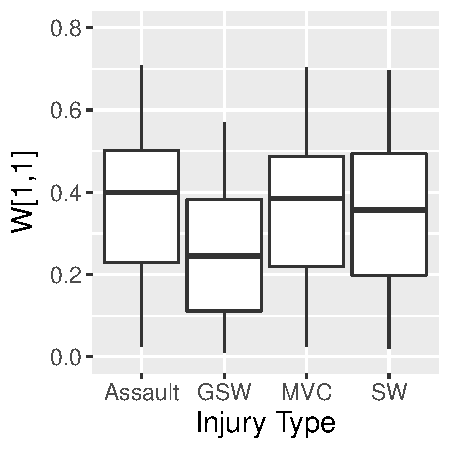
\includegraphics[width=\textwidth]{shrinkageSep.pdf}
	\label{fig:sparsePosteriors}
    \caption{Posterior intervals for elements of $W$ in sparse PCA.}\label{fig:ccaResults}
\end{figure}

%%%%%%%%%%%%%%%%%%%%%%%%%
\subsection{Coagulopathy using hierarchical subspace models}
Include figure for CCA probabilistic graphical model.

\begin{figure}
    \centering
    \begin{subfigure}[b]{0.3\textwidth}
        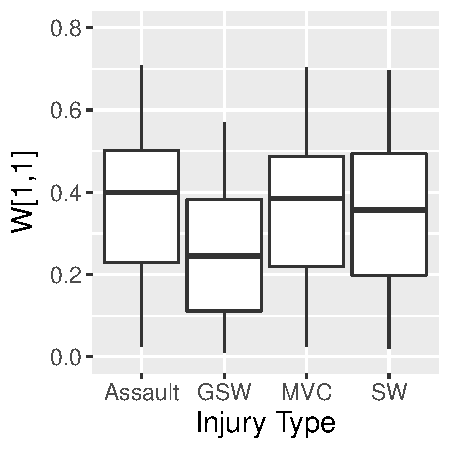
\includegraphics[width=\textwidth]{shrinkageSep.pdf}
        \caption{}
        \label{fig:nonHierPosteriors}
    \end{subfigure}
    ~ %add desired spacing between images, e. g. ~, \quad, \qquad, \hfill etc. 
      %(or a blank line to force the subfigure onto a new line)
    \begin{subfigure}[b]{0.3\textwidth}
        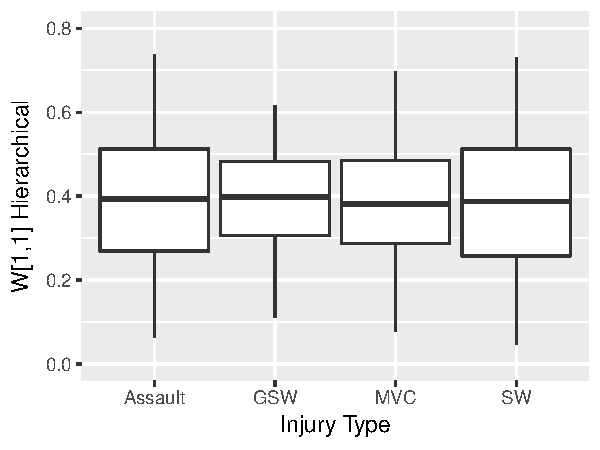
\includegraphics[width=\textwidth]{shrinkageHier.pdf}
        \caption{}
        \label{fig:hierPosteriors}
    \end{subfigure}
    ~ %add desired spacing between images, e. g. ~, \quad, \qquad, \hfill etc. 
    %(or a blank line to force the subfigure onto a new line)
    \begin{subfigure}[b]{0.3\textwidth}
        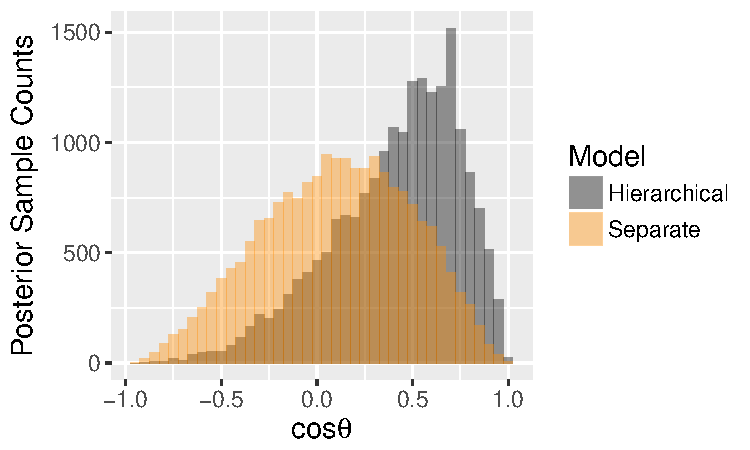
\includegraphics[width=\textwidth]{posteriorCosAngle.pdf}
        \caption{}
        \label{fig:posteriorCosAngle}
    \end{subfigure}
    \caption{Inferences for Hierarchical CCA model.}\label{fig:ccaResults}
\end{figure}

%%%%%%%%%%%%%%%%%%%%%%%%%
\subsection{School Network}
Show $W$ for each of the three states then posterior probabilities of what state you're in. Show probabilistic graphical model. Point how this can be used for disease networks and also recognizing states in fMRI data.

%%%%%%%%%%%%%%%%%%%%%%%%%
\section{Discussion}
%%%%%%%%%%%%%%%%%%%%%%%%%

\subsubsection*{Acknowledgments}

Use unnumbered third level headings for the acknowledgments. All
acknowledgments go at the end of the paper. Do not include
acknowledgments in the anonymized submission, only in the final paper.

%%%%%%%%%%%%%%%%%%%%%%%%%
%%%%%%%%%%%%%%%%%%%%%%%%%
%%%%%%%%%%%%%%%%%%%%%%%%%
\bibliographystyle{plainnat} % or try abbrvnat or unsrtnat
\bibliography{paperDatabase} % refers to example.bib

%%%%%%%%%%%%%%%%%%%%%%%%%
\section*{Appendix}
%%%%%%%%%%%%%%%%%%%%%%%%%





\subsection{Reduction Matrices}

\[
R_{ij} := 
\begin{blockarray}{cccccccccccc}
 & & & i &  & & & j & & \\
\begin{block}{(ccccccccccc)c}
  1 &  &  &  &  & & & &  & & &  \\
   & \ddots &  &  & & & & &  & & &  \\
   &  & 1  &  &  & & & &  & & & \\
   & & & \cos \theta_{ij} &  & &  & -\sin \theta_{ij} &  & & & i \\
   & & & & 1  & &  & &  & & & \\
   & & &  & & \ddots  &  & &  & & &  \\
   & & &  & & & 1 & &  & & &  \\
   & & & \sin \theta_{ij}  &  & &  & \cos \theta_{ij} &  & & & j \\
   & & &  &  & &  & & 1 & & & \\
   & & &  &  & &  & & & \ddots & & \\
      & & &  &  & &  & & & & 1 & \\
\end{block}
\end{blockarray}
 \]

\begin{equation}
R_{12}^{-1} Y 
=
R_{12}^{-1}
\begin{pmatrix}
y_{11} & y_{12} & \cdots & y_{1p}\\
y_{21} & y_{22} & \cdots & y_{2p}\\
y_{31} & y_{32} & \cdots & y_{3p}\\
\vdots & \vdots & \vdots & \vdots\\
y_{p1} & y_{p2} & \cdots & y_{pp}\\
y_{p+1,1} & y_{p+1,2} & \cdots & y_{p+1,p}\\
\vdots & \vdots & \vdots & \vdots\\
y_{n1} & y_{n2} & \cdots & y_{np}\\
\end{pmatrix}
=
\begin{pmatrix}
* & * & \cdots & *\\
0 & * & \cdots & *\\
y_{31} & y_{32} & \cdots & y_{3p}\\
\vdots & \vdots & \vdots & \vdots\\
y_{p1} & y_{p2} & \cdots & y_{pp}\\
y_{p+1,1} & y_{p+1,2} & \cdots & y_{p+1,p}\\
\vdots & \vdots & \vdots & \vdots\\
y_{n1} & y_{n2} & \cdots & y_{np}\\
\end{pmatrix}.
\end{equation}

\begin{equation}
(R_{1n}^{-1} \cdots R_{13}^{-1} R_{12}^{-1}) Y 
=
\begin{pmatrix}
1 & 0 & \cdots & 0\\
0 & * & \cdots & *\\
0 & * & \cdots & *\\
\vdots & \vdots & \vdots & \vdots\\
0 & * & \cdots & *\\
0 & * & \cdots & *\\
\vdots & \vdots & \vdots & \vdots\\
0 & * & \cdots & *\\
\end{pmatrix}.
\end{equation}

\begin{equation}
(R_{2n}^{-1} \cdots R_{23}^{-1})
(R_{1n}^{-1} \cdots R_{12}^{-1}) Y 
=
\begin{pmatrix}
1 & 0 & \cdots & 0\\
0 & 1 & \cdots & *\\
0 & 0 & \cdots & *\\
\vdots & \vdots & \vdots & \vdots\\
0 & 0 & \cdots & *\\
0 & 0 & \cdots & *\\
\vdots & \vdots & \vdots & \vdots\\
0 & 0 & \cdots & *\\
\end{pmatrix}.
\end{equation}

Continuing in this fashion yields

\begin{equation}
(R_{pn}^{-1} \cdots R_{p,p+1}^{-1})
\cdots
(R_{2n}^{-1} \cdots R_{23}^{-1})
(R_{1n}^{-1} \cdots R_{12}^{-1}) Y 
=
\begin{pmatrix}
1 & 0 & 0 & 0\\
0 & 1 & 0 & 0\\
0 & 0 & \ddots & 0\\
0 & 0 & 0 & 1\\
\vdots & \vdots & \vdots & \vdots\\
0 & 0 & \cdots & 0\\
0 & 0 & \cdots & 0\\
\vdots & \vdots & \vdots & \vdots\\
0 & 0 & \cdots & 0\\
\end{pmatrix}
=
I_{np}.
\end{equation}

\section{Misc LaTeX}



%%%%%%%%%%%%%%%%%%%%%%%%%
\subsection{Givens Reductions}
%%%%%%%%%%%%%%%%%%%%%%%%%

\commentPJA{I've temporarily moved this to the misc text section, to be added back into the main exposition in a more streamlined way.}
We provide a brief exposition on Givens Reductions, which motivate the Givens Transform, then describe the Givens Transform along with relevant practical considerations.

Define $R_{ij}$ to be the $n \times n$ rotation matrix that performs a counter-clockwise rotation in the $(i,j)$-plane of $\mathbb{R}^n$, where $j > i$. In $\mathbb{R}^3$, there are three such matrices, $R_{12}$, $R_{13}$, and $R_{23}$. They perform counter-clockwise rotation of angle $\theta_{ij}$ in the $(x,y)$, $(x,z)$ and $(y,z)$ planes respectively. Rotation matrices have the following key properties:

\begin{enumerate}
\item They preserve length and angles between vectors, i.e. for two vectors $u,v \in \mathbb{R}^n$, $R_{ij} u, R_{ij} v$ are the same length as $u$ and $v$ respectively, and if $u$ and $v$ are orthogonal then so are $R_{ij}u$ and $R_{ij}v$.
\item They are invertible and their inverse is their transpose $R_{ij}^{-1} = R_{ij}^T$. Their inverse corresponds to a clockwise rotation in the $(i,j)$-plane.
\end{enumerate}

%%%%%%%%%%%%%%%%%%%%%%%%%
Now we consider an $n \times p$ matrix $Y$, with orthonormal columns. In general, the first column is a vector in $\mathbb{R}^n$ with a non-zero second element. However, we can apply an invertible clockwise rotation in the $(1,2)$-plane, $R_{12}^{-1}$, to ``zero out" the second element of the first column. Figure \ref{fig:GivensReduction} depicts this visually for a 3D vector projected on to the $(1,2)$-plane.


Similarly, we can apply consecutive rotations $R_{13}^{-1}, R_{14}^{-1}, \cdots, R_{1n}^{-1}$ to this result so that all entries of the first column besides the first element are zero. The first column of the resulting matrix, $R_{1n}^{-1} \cdots R_{13}^{-1}  R_{12}^{-1}Y$, will be the length one vector $(1 \, 0 \, \cdots \, 0)^T$ which lies entirely along the first axis. If one takes the perspective that these rotations are applied to the columns of $Y$, then with the two properties of rotation matrices we mentioned earlier, it is evident that columns 2 through $n$ must have zero in their first element because they will be orthogonal to the first column, $(1 \, 0 \, \cdots \, 0)^T$.

To ``zero out" the elements of the second column, one can similarly apply rotations $R_{23}^{-1}, \cdots, R_{2n}^{-1}$. These rotations will leave the first column and first row unaffected, as the first column no lies entirely on the 1st axis, which these rotations do not involve. Continuing in this fashion yields

\begin{equation}
\label{eq:GivensReduction}
(R_{pn}^{-1} \cdots R_{p,p+2}^{-1} R_{p,p+1}^{-1}) \cdots (R_{2n}^{-1} \cdots R_{24}^{-1} R_{23}^{-1})(R_{1n}^{-1} \cdots R_{13}^{-1}  R_{12}^{-1})Y = I_{n,p},
\end{equation}

where $I_{n,p}$ consists of the first $p$ columns of the $n \times n$ identity matrix. This process of applying consecutive rotation matrices to a matrix is known in numerical analysis as the Givens reduction \citep{meyer2000matrix}, and is applied more generally to square matrices for matrix-vector solves. In total we will have applied $(n-1)+(n-2)+\cdots+(n-p) = np -p(p+1)/2$ rotations matrices. We note that because rotation matrices are very sparse in high dimensions, multiplication by a rotation matrix is computationally much less intensive than matrix multiplication otherwise would be.

%%%%%%%%%%%%%%%%%%%%%%%%%%%%%
\subsection{Givens Transform}
Because rotation matrices are invertible, equation \ref{eq:GivensReduction} implies that we can rewrite the $n \times p$ orthonormal matrix $Y$ as the product of counter-clockwise rotation matrices and $I_{n,p}$:

\begin{equation}
\label{eq:GivensRepresentation}
Y = (R_{12} \cdots R_{1n}) \cdots (R_{23} \cdots R_{2n}) (R_{p+1,n} \cdots R_{pn}) I_{n,p}.
\end{equation}

Recall that each of the $np -p(p+1)/2$ rotation matrices have an associated  angle $(\theta_{12} \cdots \theta_{1n}) \cdots (\theta_{23} \cdots \theta_{2n}) (\theta_{p+1,n} \cdots \theta_{pn})$, that we collectively refer to as $\Theta$. In this way we have reparameterized all $n \times p$ orthonormal matrices \footnote{other than a set of measure zero we explain in the next subsection}, a constrained space, in terms of unconstrained angles \footnote{the angles are themselves constrained to lie in certain intervals e.g. $[0, \pi)$ but these sorts of constraints are routine to deal with using a one-to-one diffeomorphism between intervals and the real line e.g. the sigmoid transform}, using a transform $\Theta: V_{n,p} \to \mathbb{R}^{np -p(p+1)/2}$. We refer to \ref{eq:GivensRepresentation} as the Givens representation or Givens transform.



%%%%%%%%%%%%%%%%%%%%%%%%%%%%%
\subsubsection{Practical considerations of topology and angles}
Topologically, $V_{n,p}$ is locally equivalent to Euclidean space, but not globally equivalent, meaning it is impossible to find a one-to-one map between the Stiefel manifold and Euclidean space. Technically speaking, the Givens transform can map angles to all of $V_{n,p}$ except for a subset $S \subset V_{n,p}$, that in the $n=3, p=2$ case corresponds to a sliver when $\theta_{12} \in (-\pi, \pi)$, $\theta_{13} \in (-\pi/2, \pi/2)$, and $\theta_{23} \in (-\pi/2, \pi/2)$. Luckily this set is of measure zero (under the proper measure for the Stiefel manifold, see section \ref{differentialFormsSection}), and thus, with probability one, the orthonormal matrix that describes the true subspace our data lie in will not be in that set. 

In practice, we actually limit the angle $\theta_{12}$ to an interval of length $\pi$ rather than an integral of length $2\pi$, that traverses the entire Stiefel manifold. Examining the angles of the Givens transform makes it evident that in the latter case, two equivalent bases that are the negation of each other can be reached, resulting in a multi-modal posterior that makes sampling and VI more difficult and harder to interpret. To avoid this multi-modality using the modified integrator methods would require a mechanism to avoid boundaries, which are not as intuitively defined in the default embedded coordinates as in the Givens transform.

Lastly, we note that if the true bases lies near a pole, i.e. $\theta_{ij}$ is close to $-\pi/2$ or $\pi/2$, then posteriors will tend to be multi-modal as the region in parameter space close to the boundaries will be close to equally valid, while the region near zero, will not be valid and thus contain little probability mass. In these cases, one can simply change the chart so that $\theta_{ij} \in (0, \pi)$, creating a uni-modal posterior in the new coordinate system, and alleviating numerical issues. In Stan this is straight-forward, as one simply has to change the lower and upper bound of the angle parameter.

%%%%%%%%%%%%%%%%%%%%%%%%%%%%%
\subsubsection{Jacobian under a change of variables}
The Givens transform \ref{eq:GivensRepresentation} allows us to represent orthonormal matrices as angles $Y(\Theta)$. This in turn allows us to write probability densities $p_Y(Y)$ in terms of angles, so that we can conduct inference in an unconstrained space. It is well known in probability theory that the transform of a random variable is in general not the density of the transform, i.e. $p_\Theta(\Theta) \neq p_Y(Y(\Theta))$\citep[chapt.~2.6]{murphy2012machine}. To be more precise, densities are measured against volumes and integrated to get actual probabilities (otherwise known as probability mass). Under a transformation, densities are unaffected, but volumes (or rather the way in which volumes are measured) may change. This is important in the context of posterior inference, as not including the Jacobian adjustment would result in different priors than we intend.

Figure \ref{fig:AreaForm} depicts how samples that are uniform in the angle space are not uniform on the sphere. Samples congregate at the poles of the sphere because a patch of area in the angle space that is near the top corresponds to a very tiny patch of the sphere near the pole. In practice this would lead to posteriors that bias towards the poles, when what we really intend is a prior that is uniform on the Stiefel manifold.

For a $K$-dimensional random vector $Y$ and a transformation $f: \mathrm{supp}(Y) \to \mathbb{R}^K$ the proper way to measure probability under a transform is by multiplying by the determinant of the Jacobian of the the inverse transform:

\begin{equation}
\int p_\Theta(\Theta)\, d\Theta = \int p_Y(Y(\Theta)) |\det J_{f^{-1}}(\Theta)|\, d\Theta.
\end{equation}

In our case this poses a problem however, because an $n \times p$ orthonormal matrix is $np$-dimensional, but the Givens transform, $\Theta(Y)$, maps this set to a $np - p(p+1)2$-dimensional set. In this more general scenario, one can not simply take the determinant of the Jacobian as the volume morphing factor, because the Jacobian is not even square and hence the determinant is undefined. To obtain the correct factor one must appeal to the calculus of differential forms. 

%%%%%%%%%%%%%%%%%%%%%%%%%%%%%
\subsubsection{Differential forms}\label{differentialFormsSection}

We offer an intuitive high-level overview of differential forms. For a thorough account we recommend \citet{muirhead2009aspects}, \citet{edelman200518}, or any standard text in differential geometry. The simplest non-trivial example of differential-forms between spaces of different sizes arises when trying to measure probablity using spherical coordinates. Spherical coordinates give us a map from $\mathbb{R}^2$ to the sphere, $(\theta, \varphi) \mapsto (x(\theta,\varphi), y(\theta,\varphi), z(\theta,\varphi))$. Although a sphere lies in 3-D space, if we have a density $p_\mathrm{Euc}(x,y,z)$ on the sphere, the ``natural'' way to measure the probability of a spherical random variable falling within some area on the surface of that sphere is by first covering that area with tiny rectangles tangent to the sphere, taking the average density of each rectangle, multiplying that density by the area of that rectangle, and summing over the resulting products. The probability of the random variable falling within that area is defined to be the limit of that result as the size of the rectangles go to zero. Area forms, or two-forms can be thought of as these infitessimal rectangles. They are written as the wedge product of two differentials, e.g. $dx \wedge dy$, and they are objects that are inserted into integrals to obtain measures. Differential forms form (no pun intended) a vector space useful for measuring areas and high-dimensional volumes. For example, the area forms on a sphere can be written as a linear combination of the standard-basis two forms

\begin{equation}
\label{eq:EuclideanAreaForm}
a(x,y,z)\, dx \wedge dy + b(x,y,z)\, dx \wedge dz + c(x,y,z)\, dy \wedge dz.
\end{equation}

One can then integrate this over a sub-area of the sphere to obtain the measure of that sub-area. The beauty of differential forms is that a different coordinate system such as polar coordinates, simply correspond to using a different basis for representing forms, which again are vectors. In fact writing a form in a different bases simply involves taking partial derivatives, e.g. $dx = (\partial x/\partial \theta) \, d\theta + (\partial x/ \partial \varphi) \, d\varphi$. If we substitute the forms in the angle bases in to \ref{eq:EuclideanAreaForm} and simplify using the well-defined anti-symmetric and distributive properties of wedge products and differential forms (see \citep{muirhead2009aspects}), we obtain a proper area-form \ref{eq:EuclideanAreaForm} in spherical coordinates, $S(x(\theta, \varphi),y(\theta, \varphi),z(\theta, \varphi))\, d\theta \wedge d\varphi$, that can then be integrated using a double integral in polar coordinates. The absolute value of this area-form evaluated at some point specified in angle coordinates, $(\theta_0, \varphi_0)$, intuitively measures how much the area of tiny square in angle space gets shrunk or stretched when the area is mapped to an area on the sphere.

Analogously, we can measure volumes on the Stiefel manifold. For $n \times p$ orthonormal matrices, there are only $np-p(p+1)/2$ free parameters and so the proper form to measure sets of orthonormal matrices is in fact a $np-p(p+1)/2$-form. For an orthonormal, $n \times p$ matrix, $Y$, we can find an orthonormal $n \times n$ matrix $G$ such that $G^T Y = I_{n,p}$. In fact $G$ just comes from the product of the appropriate rotation matrices that comes from the Givens Reduction \ref{eq:GivensReduction}. \citet{muirhead2009aspects} shows that the correct form comes from wedging the elements of the $n \times p$ matrix $G^T dY$ that lie below the diagonal i.e.

\begin{equation}
\label{eq:WedgeForm}
\bigwedge_{i=1}^p \bigwedge_{j=i+1}^n G_j^T\, dY_i
\end{equation}

where $G_j$ is the $j$th column of $G$ and $Y_i$ is the $i$th column of $Y$. To obtain the form in angle coordinates we simply obtain $dY$ in angle coordinates. $dY_i$ can be obtained in terms of the angle coordinates by the following relationship, $dY_i = J_{Y_i}(\Theta)\, d\Theta$, where $J_{Y_i}$ is the Jacobian of $Y_i$ with respect to the angle coordinates. Once we obtain the form \ref{eq:WedgeForm} in terms of the angle coordinates, the result is a wedge product of $np-p(p+1)/2$ vectors that are $np-p(p+1)/2$ dimensional, which reduces to the determinant of these vectors aligned side by side as a $np-p(p+1)/2 \times np-p(p+1)/2$ matrix. This determinant is analogous to and serves the same purpose as Jacobian adjustment that comes from transforming random variables. We can insert it in to the log-probability of a model to avoid the sort of unintended sampling behavior depicted in Figure \ref{fig:AreaForm}. We incorporate the form \ref{eq:WedgeForm} in to the log-probability of all of our Stan examples.

%%%%%%%%%%%%%%%%%%%%%%%%%
\subsection{A hierarchical PPCA model for fMRI data}
To illustrate the usefulness of GT-PPCA in a real-life setting, we applied it to a brain fMRI dataset and fit a hierarchical model using VI in Stan. We obtained 90-dimensional fMRI scans of five human subjects under an ``active" condition where subjects were asked to perform a task, and a ``resting" condition where subjects were not given any tasks or instructions. Each of the 90 dimensions corresponds to an activity level of a distinct area of the brain. From the data scientists wanted to discern whether fMRI activities were markedly different under the active and resting tasks.

It is well known that brain fMRI data is highly correlated so that our high dimensional data actually lies on some low dimensional subspace. In preliminary analysis we saw that the first principal component was highly tied to brain region 78 when subjects were in the resting state. We sought to test whether under the two states the first principal component had differing correlations to this brain region.  Examining the posterior distribution of the GT parameter $\theta_{1,78}$ we can intuitively understand how correlated with the 78th brain region the first component is. Drawing from our intuition from Figure \ref{fig:GivensReduction}, when this parameter is close to $\pi/2$ or $-\pi/2$ then the first component is highly correlated to the 78th brain region. Figure \ref{fig:fmriHier} show posterior estimates of this angle parameter, $\theta_{1,78}$, for our five subjects under the two states. While it seems as though the resting state is individually higher for this parameter, it is not clear whether this relationship is statistically significant.

A-priori, we know our subjects will have similar principal components when in the resting states and different, but also similar to each other, principal components in the active state. To reflect this prior knowledge we place a truncated normal prior over $\theta_{1,78}^{i}, \, i = 1,\cdots, 5$, and estimate the hyper-parameters $\mu_0, \sigma_0$ of this prior for the active and resting state respectively. Not including the hierarchical prior is a special case of this where the hierarchical prior is completely flat, i.e. $\sigma_0 = \infty$, so that if there is a shared information between subjects our model can pick it up, and if there is not our estimates will be unaffected. Figure \ref{fig:fmriHier} shows posterior estimates for $\theta_{1,78}^{i}$, after we used a hierarchical prior on each respective state. The hierarchical prior has the regularization effect of shrinking together estimates in the two respective states, as information about one individual in the resting state tells us information about other individuals in the resting state.


\begin{figure}
    \centering
    \begin{subfigure}[b]{0.3\textwidth}
        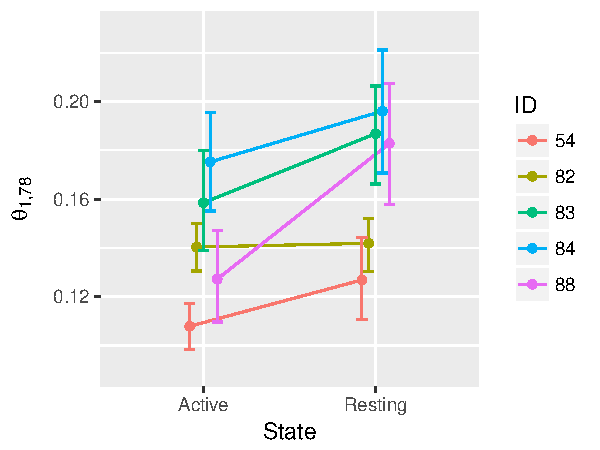
\includegraphics[width=\textwidth]{fmri.pdf}
        \caption{}
        \label{fig:fmri}
    \end{subfigure}
    ~ %add desired spacing between images, e. g. ~, \quad, \qquad, \hfill etc. 
      %(or a blank line to force the subfigure onto a new line)
    \begin{subfigure}[b]{0.3\textwidth}
        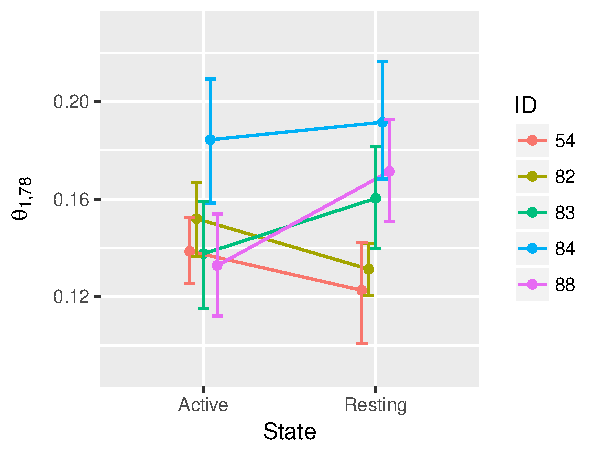
\includegraphics[width=\textwidth]{fmriHier.pdf}
        \caption{}
        \label{fig:fmriHier}
    \end{subfigure}
    ~ %add desired spacing between images, e. g. ~, \quad, \qquad, \hfill etc. 
    %(or a blank line to force the subfigure onto a new line)
    \begin{subfigure}[b]{0.3\textwidth}
        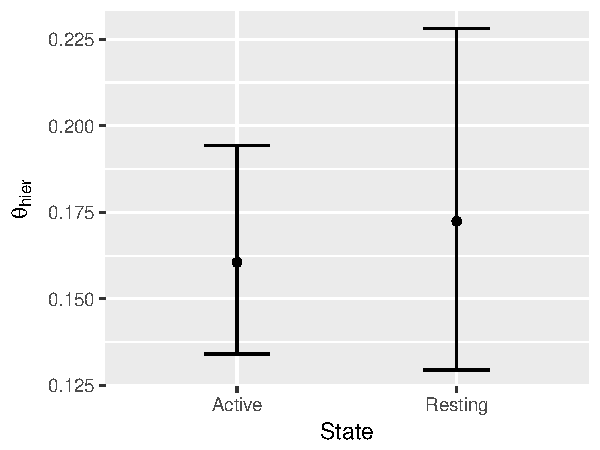
\includegraphics[width=\textwidth]{hierMean.pdf}
        \caption{}
        \label{fig:hierMean}
    \end{subfigure}
    \caption{Inferring a hierarchical subspace model for fMRI data. (a) Individual posterior estimates of Givens Transform angle $\theta_{1,78}$. (b) Hierarchical estimates. (c) Posterior mean of hierarchical mean parameter.}\label{fig:fmri}
\end{figure}

Finally, to test our original hypothesis we compared the posterior distribution of $\mu_0^{\mathrm{resting}}$ and $\mu_0^{\mathrm{active}}$ in Figure \ref{fig:hierMean}. While the posterior median of $\mu_0^{\mathrm{resting}}$ is lower, confidence intervals indicate that we would need more data to be able to conclude this with confidence, a conclusion that would be difficult to discern in a non-probabilistic framework.



\end{document}
